\documentclass{scrartcl}

% Bibliography Preamble
\usepackage[backend=biber,style=apa,sorting=none]{biblatex}
\addbibresource{Design-Document.bib}
\let\cite\textcite
\let\citep\autocite

% Graphic / Figure Preamble
\usepackage{graphicx}
\graphicspath{{img/}}

\begin{document}
\author{Charlotte Ward}
\title{ {\huge Cybersky - Design Document} \\ {\small Shoot 'Em Up Game} }
\maketitle

\section{Game Rules}

\subsection{Basis}

\subsubsection{Space Invaders (1978)}

\begin{figure}[ht]
  \centering
  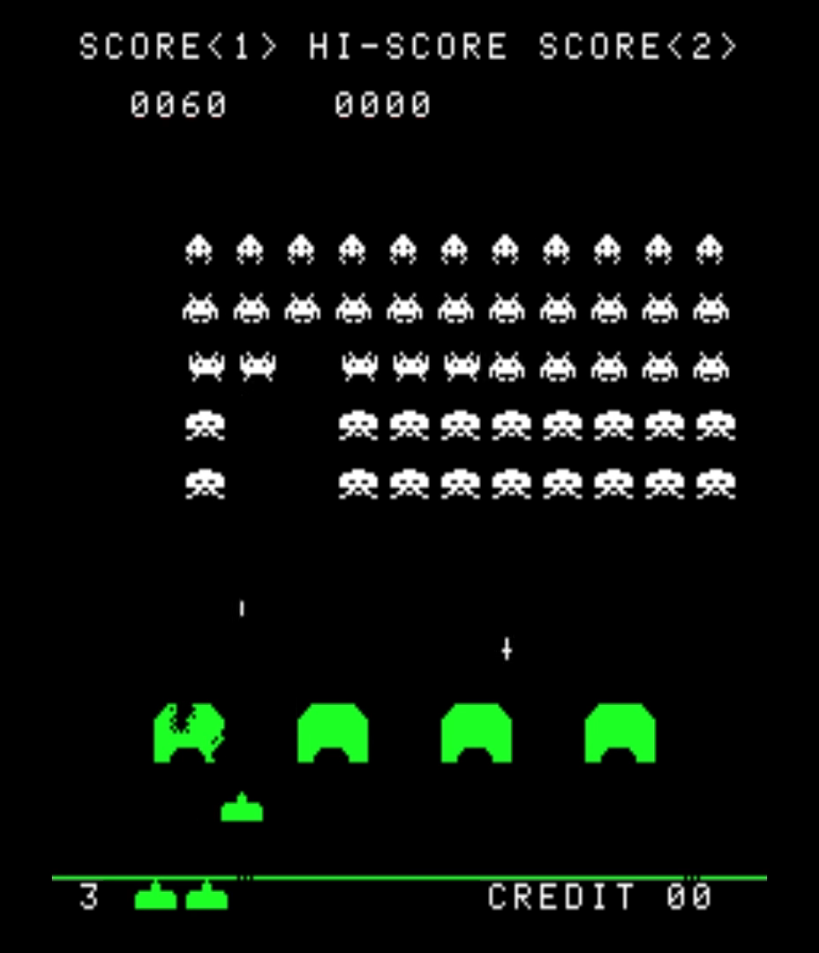
\includegraphics[width=.35\columnwidth]{SpaceInvaders.png}
  \caption[\textit{Space Invaders}]{\textit{Space Invaders} (1978) Gameplay Still from \cite{Youtube001}}
\end{figure}

Released in 1978 as an Arcade game, only 6 years after the initial release of \textit{PONG}, \textit{Space Invaders} pionered the genre of Fixed Shooter games in the arcade form factor, later becoming the basis for Shoot 'Em Up games. With the arcade game industry going through something of a 'Golden Age' \citep{BMIGaming001}, \textit{Space Invaders} was at the forefront of the industry's growth, reaching number 2 of all time in terms of sales and revenue \citep{USGamer001}.

With Shoot 'Em Up games mimicing many of the features and game rules utilised by \textit{Space Invaders}, it's important to take a look back and see exactly how the game worked and what the source of it's popularity is.

\begin{figure}[ht]
  \centering
  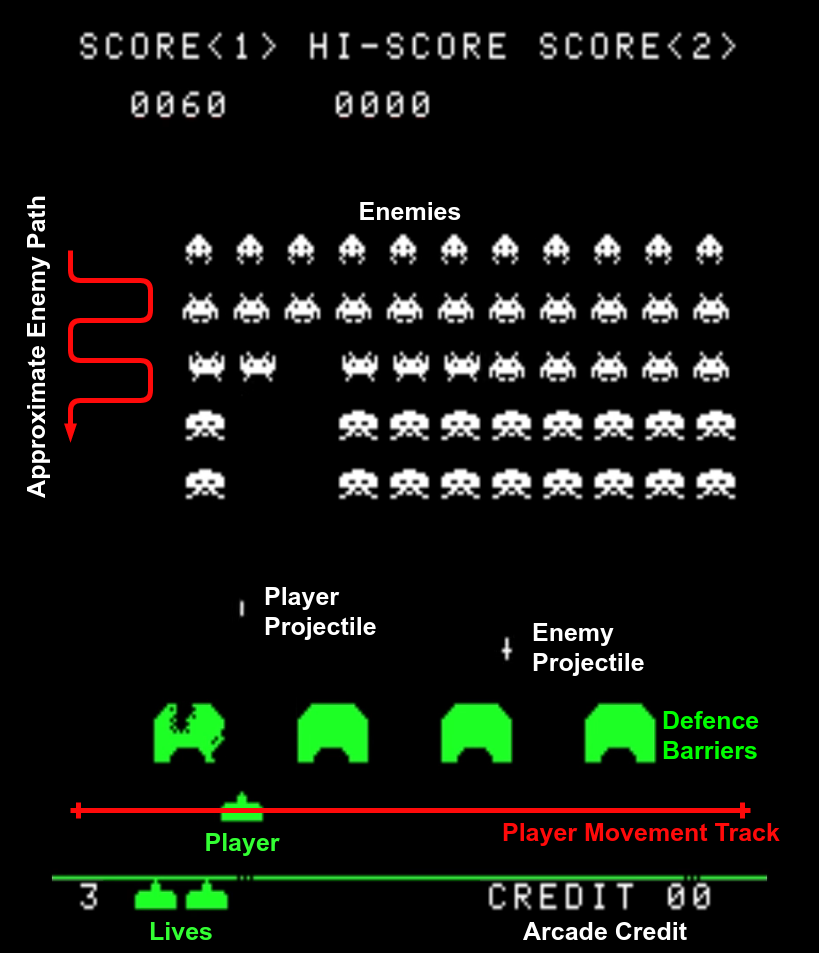
\includegraphics[width=.6\columnwidth]{SpaceInvadersBreakdown.png}
  \caption[\textit{Space Invaders}]{Modified \textit{Space Invaders} (1978) Gameplay Still from \cite{Youtube001}}
\end{figure}

This figure annotates some of the core elements in the gameplay of \textit{Space Invaders}. These elements will become important moving forward, as the Shoot 'Em Up (hereby referred to as Shmup) genre develops alongside games as a whole. These key points include:

\begin{itemize}
  \item The player can move from left to right, using an invisible track to dictate the bounds of movement.
  \item The player can fire projectiles from their player object, which fly upwards and don't move horizontally. When they hit an enemy that enemy is destroyed, and the score increments upwards.
  \item The enemies are grouped together, and follow a set path. At certain intervals, they fire projectiles towards the player, which must be avoided. Failure to avoid a projectile results in losing a life.
  \item There are barriers which can block player or enemy projectiles, but are damaged whenever they do. They can be removed completely with enough projectiles. They serve as a somewhat unreliable defence system, as the player can hide under them if needed. They also increase gameplay complexity by forcing the player to consider when and where they can fire.
\end{itemize}

\subsubsection{Galaxian (1979)}

\begin{figure}[ht]
  \centering
  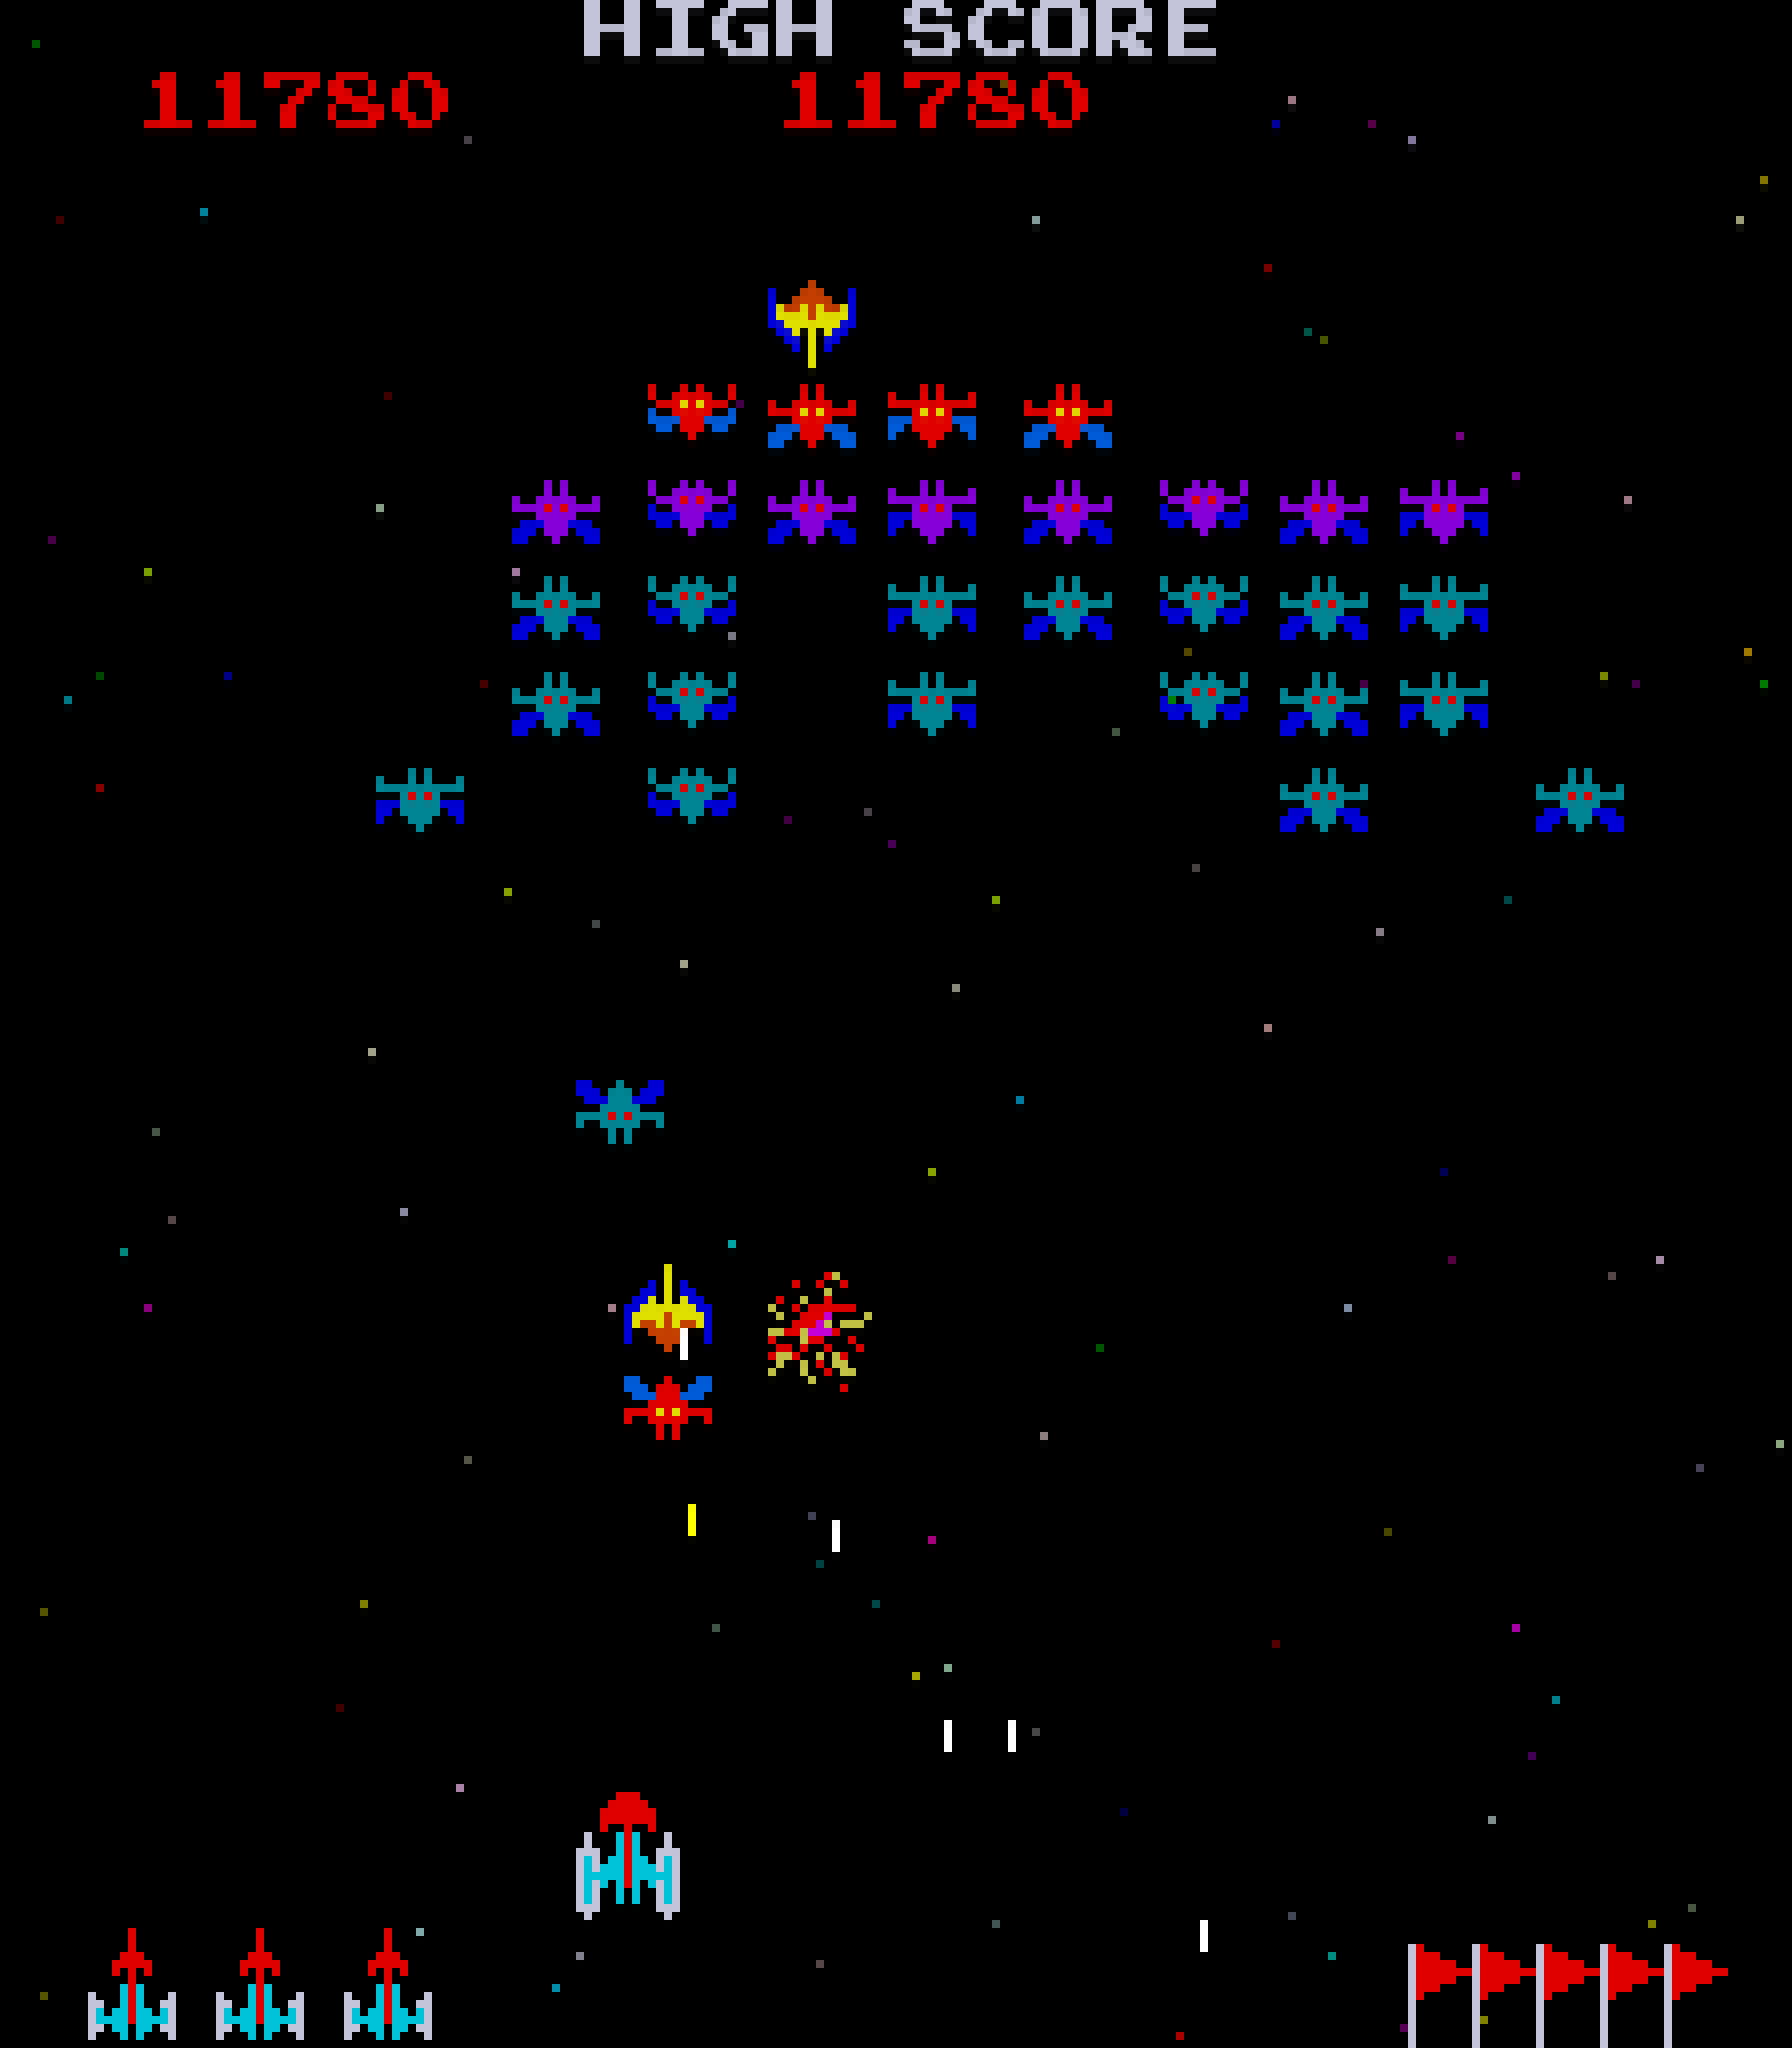
\includegraphics[width=.6\columnwidth]{Galaxian.png}
  \caption[\textit{Galaxian}]{\textit{Galaxian} (1979) Gameplay Still by \cite{Wikimedia001}}
\end{figure}


Released only a year after \textit{Space Invaders}, \textit{Galaxian} (1979) further extends the Fixed Shooter genre, improving upon \textit{Space Invader}'s successes; many of the core features remain the same, with a large group of enemies at the top of the screen, and a fixed track for player movement. The projectile system remains the same additionally, with both the player's projectiles and enemy projectiles functioning similarly.

The main differences between the two games come from differences in the visual design, gameplay complexity and overall changes in the arcade cabinet itself \citep{Youtube002}. While it's difficult to directly compare the hardware included in arcade cabinets, it's clear that the complexity involved in the game \textit{Galaxian} far outweighs that of \textit{Space Invaders}:

\begin{itemize}
  \item \textit{Galaxian} has an improved colour screen, with multi-coloured sprites.
  \item The game features a scrolling background with stars that sparkle.
  \item Enemies have animated sprites, improving on \textit{Space Invader}'s simple sprites.
\end{itemize}

Many of these differences are only clear looking at gameplay footage, but the improved design additionally is demonstrated in gameplay. For example, the gameplay revolves around an endless mode, where there's no set amount of enemies. As 'waves' of enemies are defeated, new waves turn up afterwards. This kind of gameplay is somewhat cyclical, with the core gameplay loop involving defeating batches of enemies, then progressing onto a new batch.

Additionally, the individual 'aliens' that show up in a wave can break off and fly towards the player, firing projectiles at the same time. The gameplay becomes much more hectic because of this, with many things happening on screen at once. This is an improvement on Space Invaders, where very little may be happening in a given moment. The fact that Galaxian has such a cult following and recieved so many ports should speak to the fact that this style of gameplay is popular, if striking a different target audience to Space Invaders \citep{GiantBomb001}.

\subsubsection{Ikaruga (2001)}

\begin{figure}[ht]
  \centering
  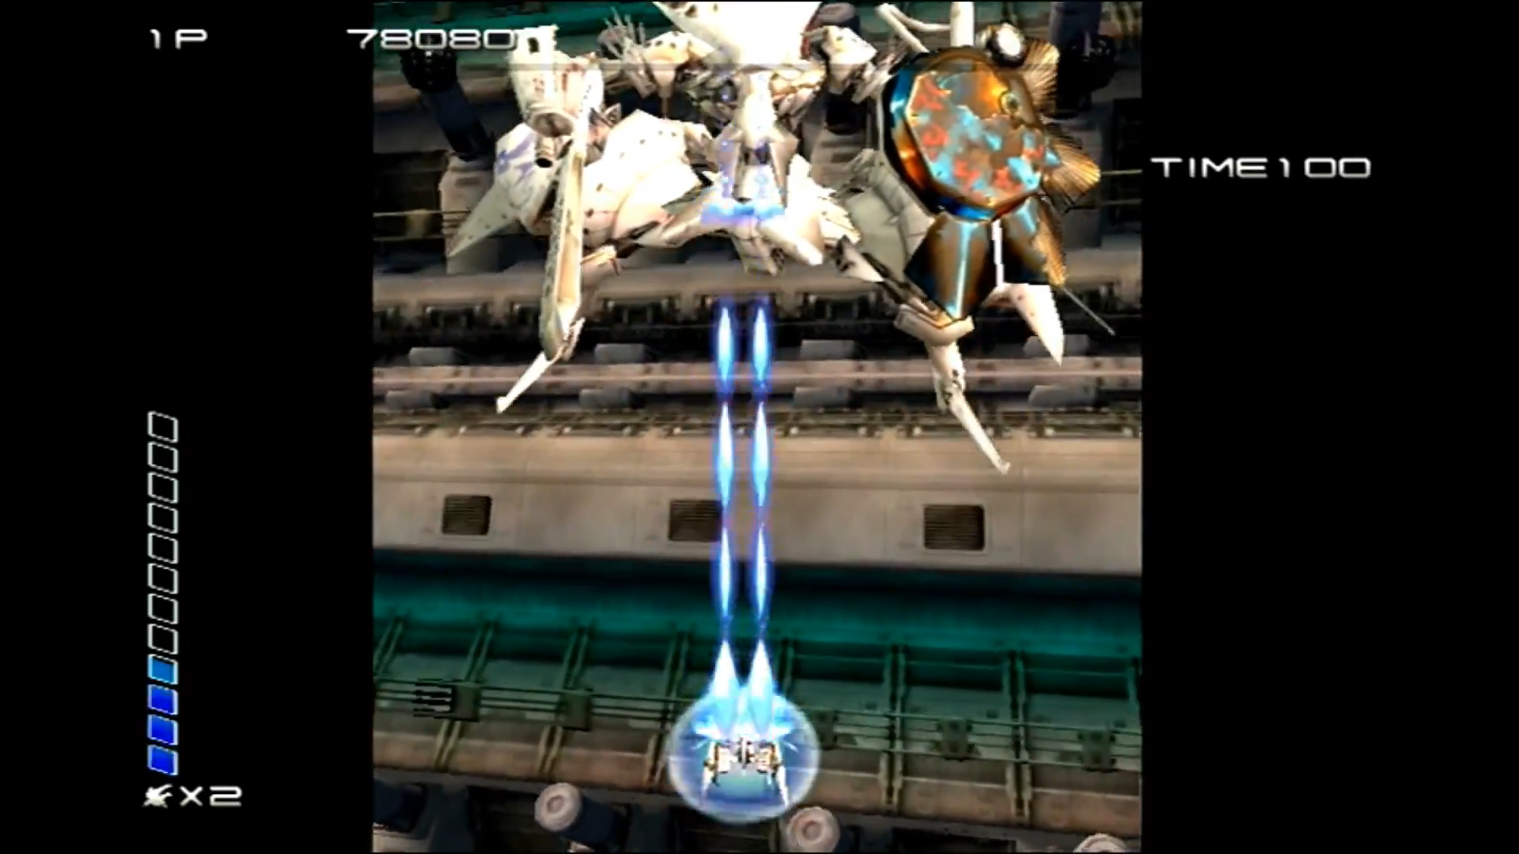
\includegraphics[width=.7\columnwidth]{Ikaruga.png}
  \caption[\textit{Ikaruga}]{\textit{Ikaruga} (2001) Gameplay Still by \cite{Youtube003}}
\end{figure}

Skipping forward a few decades, \textit{Ikaruga}, originally released in 2001, expands further upon the established gameplay rules for Shmups, with clear inspiration taken from Galaxian in the implementation of movement systems and overall gameplay. The game itself recieved a moderate following, finding the most success as a cult classic within the Bullet Hell fandom, being widely regarded as one of the best Shmups available \citep{GiantBomb002}.

While it's true that the average scene in \textit{Ikaruga} has far more going on, staying true to the moniker of Bullet Hell, both games are still relatively similar. If you boil the two games down to their core elements, not much has changed. The primary differences relate to the movement system that the player has, as well as some extra mechanical depth that comes from a toggle that the player can use.

The movement system in \textit{Ikaruga} is two dimensional, allowing the player to move forward and backward as well as left and right. I believe that the reasoning behind this relates to the player's ability to dodge attacks, making the positioning that the player can utilise much more interesting and deep by literally adding another dimension to it.

The other main mechanic that's added by \textit{Ikaruga} is a toggle that switches the player between a 'light mode' and a 'dark mode'. This is a mechanic that's mirrored in the gameplay scene, with attacks coming from enemies fitting into one of these two groups. This mechanic allows for the player to have additional control over the scene, letting them choose which kind of attack to avoid or intercept. Again, this contributes to the mechanical depth of the game, raising the skill ceiling, which is exactly what fans of the Bullet Hell type of Shmup enjoy.

\subsection{Design}

With the historical basis of Shmups in mind, it's clear that a few elements fit in quite well with the overall structure of a mobile game. All of the games explored feature a display that is taller than it is wide, which lends itself well to the form factor that a mobile phone has. Additionally, they retain simple-yet-complex mechanics for movement and interaction, which fits very well with the more simple interface of a touch-screen. Using this knowledge, it's possible to design a simple wireframe version of the game \textit{Cybersky}.

\begin{figure}[ht]
  \centering
  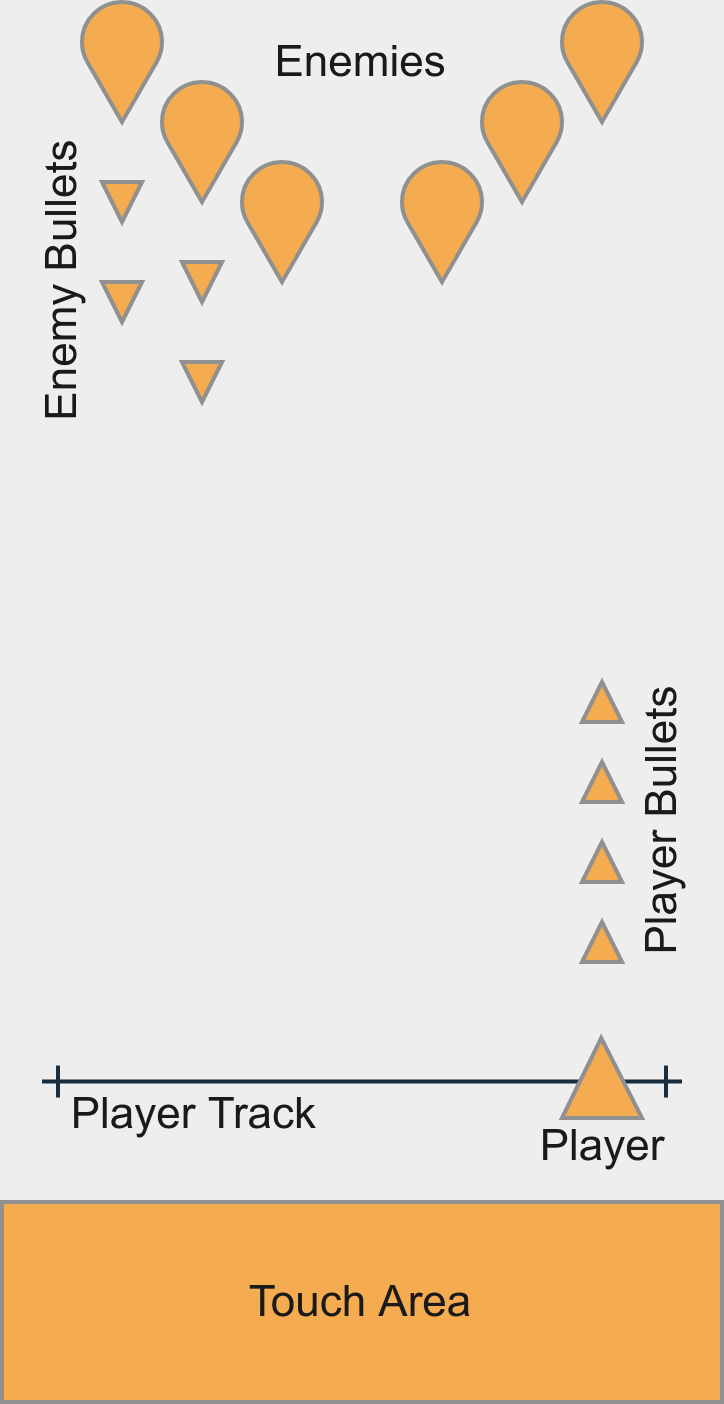
\includegraphics[width=.3\columnwidth]{concept1.png}
  \caption[\textit{Cybersky}]{\textit{Cybersky} Scene Wireframe}
\end{figure}

Figure 5 illustrates the overall design concept, showing the player on a track allowing for horizontal movement, as well as the bullets that the player can fire. Additionally, it shows a small set of enemies at the top of the screen. Borrowing elements from \textit{Galaxian} and \textit{Ikaruga}, I'd like for the player to have to dodge enemies, using the touch area at the bottom of the screen to control the horizontal position of the player element.


According to \cite{Techlector001}, phone aspect ratios fall into three major categories: 16:9, 18:9 and 19:9. The former ratio is described as the most common, being in use since around 2010. This ratio is also common in computer displays.

Phone screen sizes in the United Kingdom. \citep{DeviceAtlas2019}

\begin{tabular}{ c c c c }

  Place & Screen resolution & Share   & Aspect Ratio \\

  1.    & 750x1334          & 24.35\% & 9:16         \\

  2.    & 1080x1920         & 17.97\% & 9:16         \\

  3.    & 1440x2960         & 13.54\% & 9:18.5       \\

  4.    & 640x1136          & 7.30\%  & 9:16         \\

  5.    & 720x1280          & 7.29\%  & 9:16         \\
\end{tabular}

\paragraph{}

Using this data, it's unclear exactly how prevalent the newer, taller screen sizes are in the general market. This data doesn't necessarily represent my target audience, and as such may skew the result towards a different value.

\section{Scoring}

\section{Reward Mechanics}

\printbibliography

\end{document}
